\documentclass[tikz,border=5pt]{standalone}

\usepackage[utf8]{inputenc}
\usepackage[T1]{fontenc}
\usepackage{tikz}
\usetikzlibrary{positioning,calc,shapes,arrows,shapes.multipart,arrows.meta}

% Define block styles
\tikzset{
   papDecision/.style = {
         diamond,
         draw, 
         text width = 20 mm, 
         align = center, 
         text badly centered,
         inner sep = 1 pt,
         font=\ttfamily,
         %line width = 1,
         minimum width = 30mm,
         minimum height = 7mm,
      },
   papStart/.style = {
         rectangle,
         draw, 
         align = center, 
         text width = 3cm, 
         text badly centered,
         inner sep = 4 pt,
         rounded corners=10pt,
         font=\ttfamily,
         %line width = 1,
         minimum width = 30mm,
         minimum height = 7mm,
      },
   papEnd/.style = {
         rectangle,
         draw, 
         align = center, 
         text width = 3cm -2*\pgfkeysvalueof{/pgf/inner xsep}, 
         text badly centered,
         inner sep = 4 pt,
         rounded corners=10pt,
         font=\ttfamily,
         %line width = 1,
         minimum width = 30mm,
         minimum height = 7mm,
      },
   papData/.style = {
         trapezium,
         draw, 
         align = center, 
         text width = 1.5cm,
         text badly centered,
         inner sep = 4 pt,
         trapezium left angle=70,
         trapezium right angle=110,
         font=\ttfamily,
         %line width = 1,
%         minimum width = 30mm,
         minimum height = 7mm,
      },
   papPredProc/.style = {
         draw,
         rectangle split,
         rectangle split horizontal,
         rectangle split parts = 3,
         rectangle split empty part width=-8pt,
         align = center, 
 %       text width = 4.5 em, 
         text badly centered,
 %        inner sep = 4 pt,
         font=\ttfamily,
         %line width = 1,
         minimum width = 30mm,
         minimum height = 7mm,
      },
   papProcess/.style = {
         rectangle,
         draw,
         align = center, 
         text width = 3cm, 
         text badly centered,
         %inner sep = 2 pt,
         font=\ttfamily,
         %line width = 1,
         minimum width = 30mm,
         minimum height = 7mm,
      },
   papLine/.style = {
         draw,
         -{Stealth[length=9pt,width=6pt]},
         font=\ttfamily,
         %line width = 1,
      },
}

\newcommand{\papYes}{ja}
\newcommand{\papNo}{nein}

\begin{document}

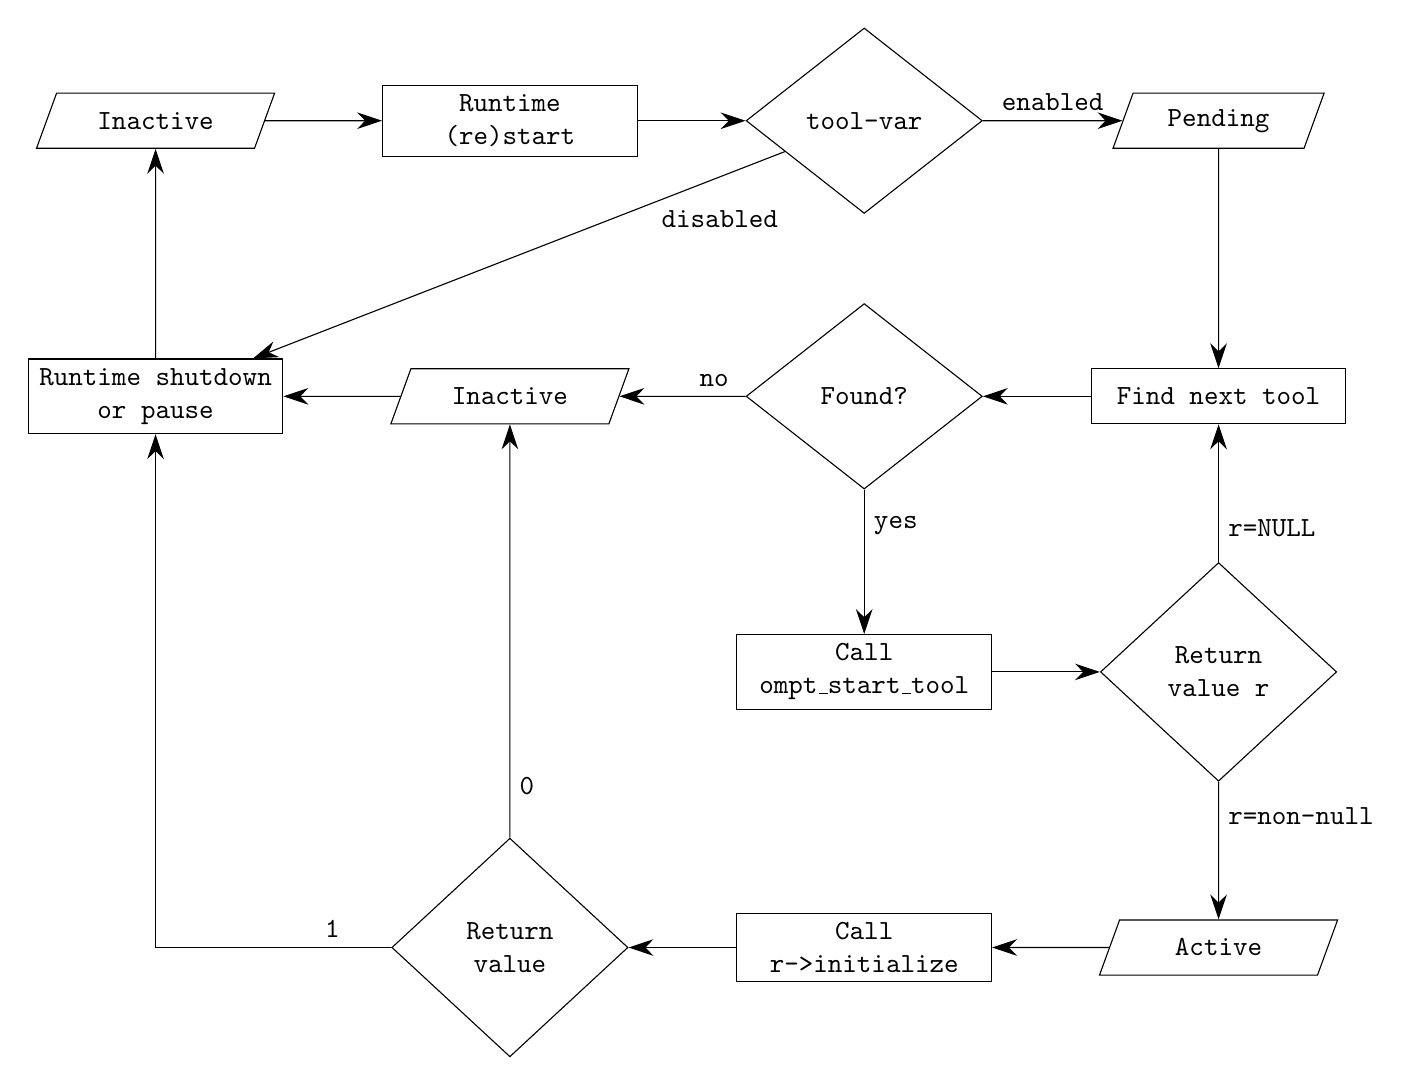
\begin{tikzpicture}[node distance = 2cm, auto]


% Place nodes
%\node [papStart] (Start1){Start};
%\node [papProcess, below of = Start1,label={[shift={(2.7,-0.6)}]\footnotesize\textit{label 1}}] (pro1){Prozess};
%\node [papData, below of = pro1,label={[shift={(3,-0.6)}]\footnotesize\textit{label 2}}](pro2){Prozess};
%\node [papDecision, below of = pro2, yshift= -9mm](dec1){Entscheidung};
%\node [papPredProc,  right of = dec1, xshift=25mm](predproc1){\nodepart{two}\shortstack{vordefinierter\\Prozess}};
%\node [papProcess, below of = predproc1,label={[shift={(2.3,-0.6)}]\footnotesize\textit{label 3}}](pro3){Prozess};
%\node [papEnd, below of = dec1, yshift= -20mm] (End) {Ende};


\node [papData] (inactive1){Inactive};
\node [papProcess, right of =inactive1 , xshift=25mm]
	(restart){Runtime (re)start};
\node [papDecision, right of =restart, xshift=25mm]
	(omptool){tool-var};
\node [papData, right of =omptool, xshift=25mm] 
	(pending){Pending};

\node [papProcess, below of =pending, yshift=-15mm] 
	(more-tools){Find next tool};

\node [papDecision, below of = more-tools, yshift=-15mm]
	(start-return){Return value r};
\node [papData, below of =start-return, yshift=-15mm] 
	(active){Active};


\node [papProcess, left of =start-return, xshift=-25mm] 
	(ompt-start-tool){Call ompt\_start\_tool};

\node [papDecision, left of =more-tools, xshift=-25mm]
	(found){Found?};
\node [papData, left of =found, xshift=-25mm] 
	(inactive2){Inactive};
\node [papProcess, below of =inactive1, yshift=-15mm] 
	(shutdown){Runtime shutdown or pause};

\node [papProcess, left of =active, xshift=-25mm] 
	(ompt-init){Call r->initialize};

\node [papDecision, left of =ompt-init, xshift=-25mm]
	(init-return){Return value};



% Place joins
%\coordinate [below of = dec1, yshift= -10mm] (join1);

\path [papLine] (inactive1) -- (restart);

\path [papLine] (restart) -- (omptool);

\path [papLine] (omptool) -- node [above] {enabled} (pending);
\path [papLine] (omptool) -- node [right, near start, yshift=-2mm] {disabled} (shutdown);

\path [papLine] (pending) -- (more-tools);

\path [papLine] (ompt-start-tool) -- (start-return);

\path [papLine] (start-return) -- node [right, near start] {r=non-null} (active);
\path [papLine] (start-return) -- node [right, near start] {r=NULL} (more-tools);

\path [papLine] (more-tools) -- (found);

\path [papLine] (found) -- node [right, near start] {yes} (ompt-start-tool);
\path [papLine] (found) -- node [above, near start] {no} (inactive2);

\path [papLine] (inactive2) -- (shutdown);

\path [papLine] (active) -- (ompt-init);

\path [papLine] (ompt-init) -- (init-return);

\path [papLine] (init-return) -| node [above, very near start] {1} (shutdown);
\path [papLine] (init-return) -- node [right, very near start] {0} (inactive2);

\path [papLine] (shutdown) -- (inactive1);


% Draw edges
%\path [papLine] (Start1) -- (pro1);
%\path [papLine] (pro1) -- (pro2);
%\path [papLine] (pro2) -- (dec1);
%\path [papLine] (dec1) -- node [right] {\papYes} (End);
%\path [papLine] (dec1) -- node [above] {\papNo} (predproc1);
%\path [papLine] (predproc1) -- (pro3);
%\path [papLine] (pro3) |- (join1);

\end{tikzpicture}

\end{document}